% Part III — Seed Selection  |  ~8 slides  |  Madrid/seahorse  |  16:9
\documentclass[aspectratio=169,10pt]{beamer}
\usetheme{Madrid}\usecolortheme{seahorse}
\usepackage{tikz}
\usetikzlibrary{arrows.meta,shapes,positioning}
\usepackage{pgfplots}\pgfplotsset{compat=1.17}
\usepackage{booktabs,amsmath,amssymb,xcolor}
\definecolor{myblue}{RGB}{0,50,130}
\definecolor{myred}{RGB}{153,0,0}
\definecolor{mygreen}{RGB}{0,100,50}
\definecolor{myorange}{RGB}{180,80,0}
\newcommand{\NHOP}{\mathrm{NHOP}}
\setbeamertemplate{navigation symbols}{}
\title[Part III: Seed Selection]{Part III — Seed Selection}
\subtitle{A Geometry-Preserving 4-Stage Pipeline}
\author{Parsa Hajiannejad}\date{2026}

\begin{document}
\begin{frame}\titlepage\end{frame}

% ----- Slide 1 ---------------------------------------------------------------
\begin{frame}{Why Seed Selection Matters}
\begin{columns}[T]
\column{0.48\textwidth}
All SMOTE-family methods synthesise \emph{from} a selected minority subset (the "seeds"). Random or boundary-based seed choice causes:
\begin{itemize}
  \item Density distortion — over-sampling sparse outlier regions
  \item Geometric infidelity — seeds don't span the true minority shape
  \item Smoothness violation — neighbouring seeds are geometrically incompatible
\end{itemize}
\vspace{6pt}
\textbf{Key insight:} NHOP $= 1-\TV$ means selecting seeds that maximise NHOP \emph{is equivalent} to minimising marginal total variation between seed-generated synthetic data and the original minority.

\column{0.50\textwidth}
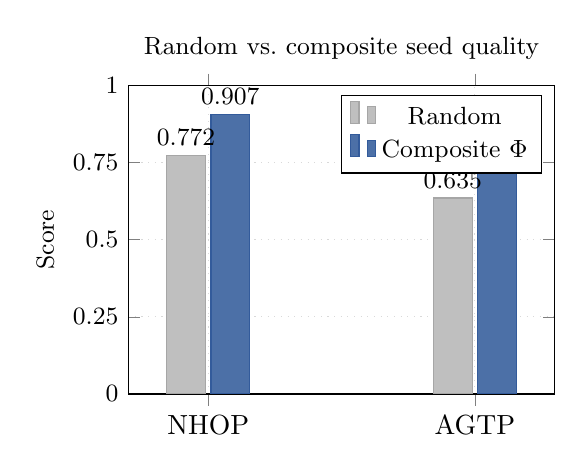
\begin{tikzpicture}
\begin{axis}[
  width=7cm,height=5.5cm,
  ybar,bar width=14pt,
  symbolic x coords={NHOP,AGTP},
  xtick=data,
  xticklabel style={font=\normalsize},
  ymin=0,ymax=1,
  ytick={0,0.25,0.5,0.75,1},
  yticklabel style={font=\small},
  ylabel={\small Score},
  title={\small Random vs.\ composite seed quality},
  title style={font=\small},
  legend style={font=\small,at={(0.97,0.97)},anchor=north east},
  enlarge x limits=0.3,
  grid=major,grid style={dotted,gray!30},
  nodes near coords,
  nodes near coords style={font=\small},
  every node near coord/.append style={/pgf/number format/.cd,fixed,precision=3}]
\addplot[fill=gray!50,draw=gray!70] coordinates {(NHOP,0.772)(AGTP,0.635)};
\addplot[fill=myblue!70,draw=myblue!80] coordinates {(NHOP,0.907)(AGTP,0.839)};
\legend{Random,Composite $\Phi$}
\end{axis}
\end{tikzpicture}
\end{columns}
\end{frame}

% ----- Slide 2 ---------------------------------------------------------------
\begin{frame}{The 4-Stage Pipeline}
\begin{center}
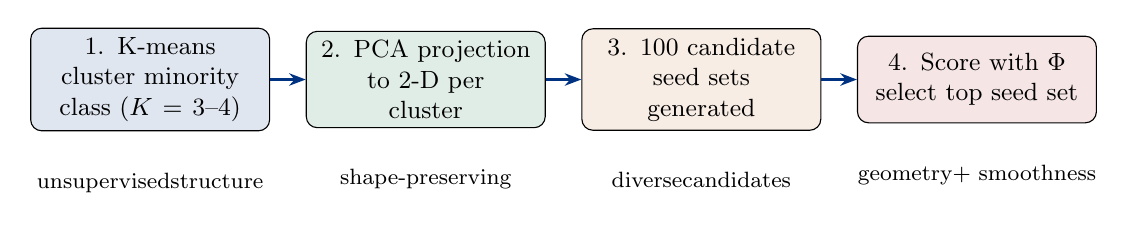
\begin{tikzpicture}[
  pnode/.style={rectangle,rounded corners=4pt,draw,fill=myblue!12,
               text width=2.8cm,align=center,font=\small,minimum height=1.1cm},
  arrow/.style={-{Stealth[length=6pt]},thick,myblue}]
\node[pnode]                   (s1) at (0,0)    {1. K-means\\cluster minority\\class ($K=3$--$4$)};
\node[pnode,fill=mygreen!12]   (s2) at (3.5,0)  {2. PCA projection\\to 2-D per\\cluster};
\node[pnode,fill=myorange!10]  (s3) at (7.0,0)  {3. 100 candidate\\seed sets\\generated};
\node[pnode,fill=myred!10]     (s4) at (10.5,0) {4. Score with $\Phi$\\select top seed set};
\draw[arrow] (s1.east)--(s2.west);
\draw[arrow] (s2.east)--(s3.west);
\draw[arrow] (s3.east)--(s4.west);
\node[font=\footnotesize,below=0.4cm of s1] {unsupervised\\structure};
\node[font=\footnotesize,below=0.4cm of s2] {shape-\\preserving};
\node[font=\footnotesize,below=0.4cm of s3] {diverse\\candidates};
\node[font=\footnotesize,below=0.4cm of s4] {geometry\\+ smoothness};
\end{tikzpicture}
\end{center}
\vspace{4pt}
\textbf{Composite criterion:}
\[
  \Phi = \underbrace{\NHOP}_{\text{distributional fidelity}}
       + \underbrace{\mathrm{AGTP}}_{\text{geometric coverage}}
       - 0.3\cdot\underbrace{\overline{\mathrm{JSD}}}_{\text{diversity penalty}}
       - 0.5\cdot\underbrace{Z}_{\text{smoothness penalty}}
\]
\textbf{PCA is essential}: AGTP drops by $0.211$ without projection ($0.839 \to 0.628$).
\end{frame}

% ----- Slide 3 ---------------------------------------------------------------
\begin{frame}{Results: Seed Quality and Downstream F1}
\begin{columns}[T]
\column{0.50\textwidth}
\textbf{Per-dataset NHOP improvement (composite vs.\ random):}
\begin{center}
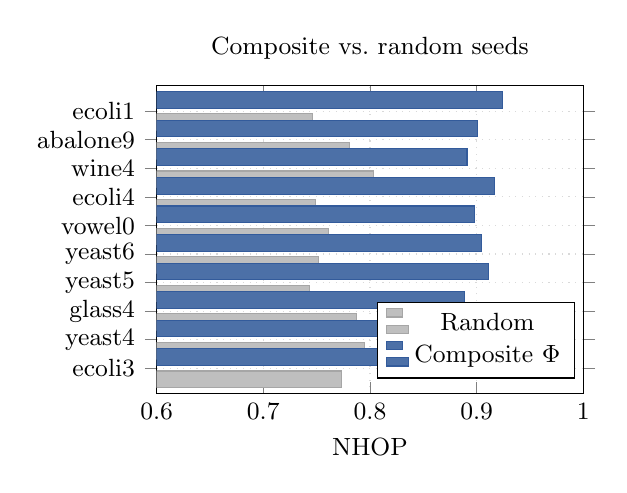
\begin{tikzpicture}
\begin{axis}[
  xbar,bar width=6pt,
  width=7cm,height=5.5cm,
  xmin=0.6,xmax=1.0,
  symbolic y coords={ecoli3,yeast4,glass4,yeast5,yeast6,vowel0,ecoli4,wine4,abalone9,ecoli1},
  ytick=data,
  yticklabel style={font=\small},
  xlabel={\small NHOP},
  xlabel style={font=\small},
  xticklabel style={font=\small},
  title={\small Composite vs.\ random seeds},
  title style={font=\small},
  legend style={font=\small,at={(0.98,0.05)},anchor=south east},
  grid=major,grid style={dotted,gray!30}]
\addplot[fill=gray!50,draw=gray!70] coordinates {
  (0.746,ecoli1)(0.781,abalone9)(0.803,wine4)(0.749,ecoli4)
  (0.761,vowel0)(0.752,yeast6)(0.743,yeast5)(0.787,glass4)
  (0.795,yeast4)(0.773,ecoli3)};
\addplot[fill=myblue!70,draw=myblue!80] coordinates {
  (0.924,ecoli1)(0.901,abalone9)(0.891,wine4)(0.917,ecoli4)
  (0.898,vowel0)(0.905,yeast6)(0.911,yeast5)(0.889,glass4)
  (0.912,yeast4)(0.907,ecoli3)};
\legend{Random,Composite $\Phi$}
\end{axis}
\end{tikzpicture}
\end{center}

\column{0.48\textwidth}
\textbf{Downstream F1 gain per classifier:}
\begin{center}
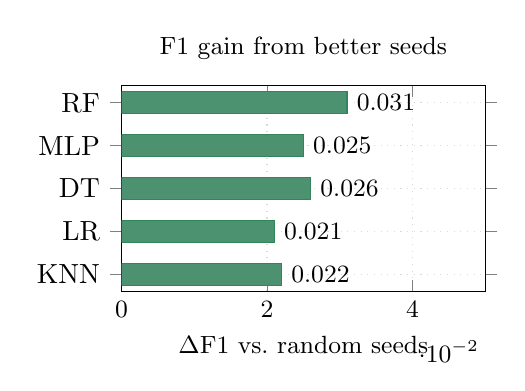
\begin{tikzpicture}
\begin{axis}[
  xbar,bar width=8pt,
  width=6.2cm,height=4.2cm,
  xmin=0,xmax=0.05,
  symbolic y coords={KNN,LR,DT,MLP,RF},
  ytick=data,
  yticklabel style={font=\normalsize},
  xlabel={\small $\Delta$F1 vs.\ random seeds},
  xlabel style={font=\small},
  xticklabel style={font=\small},
  title={\small F1 gain from better seeds},
  title style={font=\small},
  nodes near coords,
  nodes near coords style={font=\small},
  every node near coord/.append style={/pgf/number format/.cd,fixed,precision=3},
  grid=major,grid style={dotted,gray!30}]
\addplot[fill=mygreen!70,draw=mygreen!80] coordinates {
  (0.022,KNN)(0.021,LR)(0.026,DT)(0.025,MLP)(0.031,RF)};
\end{axis}
\end{tikzpicture}
\end{center}
\vspace{4pt}
Mean NHOP: $0.772 \to 0.907$ \; ($+0.135$)\\
Mean AGTP: $0.635 \to 0.839$ \; ($+0.204$)\\
Mean F1: $+0.025$ per classifier\\
Sensitivity: $+0.035$
\end{columns}
\end{frame}

\end{document}
